\section{Pangebin method}

\begin{todobox}
    Summarize thanks to an algorithm.
\end{todobox}

\begin{todobox}
    Generalize the idea of coarse-to-fine-grain approach by splitting all the objectives.
    
    \begin{enumerate}[label=\roman*.]
        \item Find max flow
        \item With flow near to max flow, find best GC score
        \item With flow near to max flow, with GC score near to best GC score, find best gene density
        \item \textbf{[Future]} With blabla, find best plasmid-type subgraph
    \end{enumerate}
\end{todobox}

Pangebin is based on the PlasBin-flow approach~\cite{manePlasBinflowFlowbasedMILP2023} and adapts its method to be applied to pan-assembly graphs.

However, Pangebin tackles the binning of the fragments with a coarse-to-fine-grain approach in three stages (each one refering to an optimization problem) iteratively applied on smaller pan-assembly graph:

\begin{enumerate}[label=\roman*.]
    \item Find the maximum coverage flow (\MCF{} problem, \Cref{meth:max_coverage_flow}) 
    \item Find the maximum GC probability score (\MGC{} problem)
    \item Find the maximum gene density score (\MGD{} problem)
\end{enumerate}

We model these three subproblems as dedicated flow formulations with Mixed Integer Linear Programming (MILP):

\begin{itemize}
    \item To keep the direction of the flow along the link-edges in \(E_\Links{}\), we define \(A_\Links{}\) as the set of link-arcs such that each link-edge is doubled according to the two directions and results in two link-arcs.
    \item We add two vertices, \(s\) and \(t\) that are respectively the source and the sink vertices in the network resulting from the augmented pan-assembly graph.
    \item The set \(\VSeed{}\) contains the vertices associated with the seed fragments. 
        The source goes into each vertex in \(\VSeed{}\), and each vertex in \(V\) goes into the sink.
        The set of link-arcs of the network \(A'_\Links{}\) equals to the union \(A_\Links{} \cup \Set{(s, v) \given v \in \VSeed{}} \cup \Set{(v, t) \given v \in V}\).
    \item The fragment coverages define the capacities.
        For each link-arc \(a \in A'_\Links{}\), we define its capacity \(\capacity{a} \in \Reals_{>0}\) equals to the minimum of the coverages of the fragments associated to the vertices. 
        In the case the link-arc connect either the source or the sink, the capacity equals the coverage of the fragment associated to the other vertex.
\end{itemize}

In what follow, we define either a fragment, a contig or an arc to be \enquote{active} if it participates in the solution, i.e. the flow passes through it.

\begin{newfeatbox}
    At the opposite of PlasBin-flow, we split each objective expression into different mono-objective functions that define different optimization problems. 
\end{newfeatbox}

\begin{todobox}
    Describe the update of the graph between the iterations (for the two problems).

    \begin{enumerate}
        \item reduce the coverage
        \item remove from the contig set the contigs for which one of its fragment has a null coverage 
    \end{enumerate}
\end{todobox}

\subsection{The Maximum Coverage-likelihood Flow problem \MCF{}}\label{meth:max_coverage_flow}

The first binning stage consists in finding a flow maximizing the use of fragment coverage.
We refer to this subproblem as the \enquote{Maximum Coverage-likelihood Flow} problem (\MCF{}).
As a coarse-grain strategy, it consists in finding a connected component explaining the coverages, large enough to contain all the fragments of the in-building solution bin.
Indeed, passing through a loop or a cycle will not change the flow value. Only maximizing the flow can lead to use a minimum of fragments.
To overcome this bias, we score the use of the fragment coverages and maximize their total.
Bellow we describe the MILP model.

\begin{newfeatbox}
    Here we maximize the coverage scores, not only the coverage flow.
\end{newfeatbox}

\begin{definition}{\MCF{} MILP variables}{milp:mcf_variables}
    \begin{itemize}
        \item \(x_i \in \Reals_{\geq 0} \, \forall i \in \Fragments{}\) denoting whether the fragment \(i\) is active or not. With the constraints it acts as a binary.
        \item \(y_a \in \Set{0, 1} \, \forall a \in A'_\Links{}\) denoting whether the link-arc \(a\) is active or not.
        \item \(f_a \in \Reals_{\geq 0} \, \forall a \in A'_\Links{}\) corresponding to the flow amount passing through the link-arc \(a\).
        \item \(F \in \Reals_{\geq 0}\) corresponding to the overall flow.
        \item \(F_a \in \Reals_{\geq 0} \, \forall a \in A'_\Links{}\) playing the role of an intermediary variable to force the flow on each link-arc to be equal to the total flow.
    \end{itemize}
\end{definition}


\begin{definition}{\MCF{} MILP constraints}{milp:mcf_constraints}

    Exactly one link-arc outs of \(s\) is part of the solution (necessary to ensure the solution induced subgraph has only one connected component):
    \begin{todobox}
        Describe why it is not sufficient to have only one connected component
    \end{todobox}
    \begin{equation}
        \sum_{a \in \Set{(s, v) \given v \in \VSeed{}}} y_a = 1
    \end{equation}
    
    The flow through a link-arc \(a \in A'_\Links{}\) is non-zero if \(a\) is active and cannot exceed its capacity: 
    \begin{equation}
        f_a \leq \capacity{a} y_a \quad \forall a \in A'_\Links{}
    \end{equation}

    The cumulative flow through a fragment \(i \in \Fragments{}\) cannot exceed its read coverage:
    \begin{equation}
        inflow(i) \leq \cov{i} \quad \forall i \in \Fragments{}
    \end{equation} 
    Where \(\displaystyle inflow(i) = \sum_{a \in A'^-_{V_t(i)} \cup A'^-_{V_h(i)}} f_a\), \(A'^-_{V_t(i)}\) and \(A'^-_{V_h(i)}\) are the sets of incoming link-arcs in \(A'_\Links{}\) for respectively the tail and the head vertices of fragment \(i\).

    The cumulative flow into a fragment \(i\) should be equal to the cumulative flow out of it. Conversely for the reverse \(i^-\):
    \begin{align}
        \sum_{a \in A'^-_{V_t(i)}} f_a & = \sum_{a \in A'^+_{V_h(i)}} f_a & \forall i \in \Fragments{} \\
        \sum_{a \in A'^-_{V_h(i)}} f_a & = \sum_{a \in A'^+_{V_t(i)}} f_a & \forall i \in \Fragments{}
    \end{align}

    The total flow value \(F\) equals to the flow out of \(s\) and into \(t\):
    \begin{align}
        F & = \sum_{a \in \Set{(s, v) \given v \in \VSeed{}}} f_a \\
        F & = \sum_{a \in \Set{(v, t) \given v \in V}} f_a
    \end{align}

    The fragments involved in an active link-arc must also be active:
    \begin{equation}
        y_{uv} \leq \min\Set{x_i, x_j} \quad \forall (u, v) \in A'_\Links{}, i = vfrag(u), j = vfrag(v) 
    \end{equation}

    An active fragment implies at least one link-arc incident to one of the its extremities is active:
    \begin{equation}
        x_i \leq \sum_{a \in A'^-_{V_t(i)} \cup A'^-_{V_h(i)}} y_a
    \end{equation}

    An active link-arc has a flow at least \(F\).
    \begin{align}
        F_a & \geq F - (1 - y_a) \max_{\substack{v \in \VSeed{} \\ i = vfrag(v)}}\Set{\cov{i}} & \forall a \in A'_\Links{} \\
        F_a & \leq F & \forall a \in A'_\Links{} \\
        F_a & \leq f_a & \forall a \in A'_\Links{} \label{const:arc_flow_at_least_total_flow}
    \end{align}
    \begin{infobox}
        The above constraints minimize the number of out link-arcs for each fragment.
    \end{infobox}
    \begin{missingproofbox}
        If several link-arcs out of a given fragment,
        then this fragment is repeated (immediate).
    \end{missingproofbox}
    \begin{questionbox}
        What is the meaning for a fragment to have a cumulative flow that is not a multiple of \(F\)?
        By keeping the flow real, can we smartly force the cumulative flow to be a multiple of \(F\)? 

        \begin{notebox}
            Because the sequencing coverage does not represent an integer number of copy of the sequenced genome.
        \end{notebox}
    \end{questionbox}

    \begin{todobox}
        Describe the connected component set of constraints.
        \begin{notebox}
            These constraints will force variables x to take value either 0 or 1
        \end{notebox}
    \end{todobox}
\end{definition}

\begin{definition}{\MCF{} MILP objective function}{milp:mcf_objective}
    The objective function aims to maximize the total coverage scores:
    \begin{equation}
        \max ~ CoverageScore
    \end{equation}
    where \(
        \displaystyle CoverageScore = %
            \sum_{i \in \Fragments{}} \parenth*{2 \frac{inflow(i)}{\cov{i}} - 1}
    \).
\end{definition}

\subsection{The Maximum GC Probability Score problem \MGC{}}\label{sec:method:mgc}

The second binning stage consists in finding a flow maximizing the GC probability scores, by fixing the coverage score flow.
We refer to this subproblem as the \enquote{Maximum GC Probability Score} problem (\MGC{}).
In the following we describe the MILP model.

\begin{definition}{\MGC{} MILP variables}{milp:mgc:variables}
  We complete \Cref{definition:milp:mcf:variables} with the following variables:
  \begin{itemize}
    \item \(GC_b \in \Set{0, 1} \, \forall b \in K\) denoting whether the plasmid GC content is in the GC content interval \(b\) or not.
    \item \(\fraggc{i}{b} \in \Reals_{>=0} \, \forall (i, b) \in \Fragments{} \times K\) denoting whether the fragment \(i\) is active and the plasmid GC content is in the interval \(b\) or not. With the constraints it acts as a binary.
  \end{itemize}
\end{definition}

\begin{definition}{\MGC{} MILP constraints}{milp:mgc:constraints}
  To the constraints in \Cref{definition:milp:mcf:constraints} we add the following:

  \phantom{text}
  The coverage score must be near to the optimal coverage score \(\Phi{}\) found in \MCF{}:
  \begin{equation}
    \gamma_1 \Phi \leq CoverageScore \quad \gamma_1 \in (0.5, 1] % chktex 9
    \cstlabel{mgc:cst:coverage_score_near_optimal} % chktex 25
  \end{equation}

  The plasmid GC content is in exactly one GC content interval \(b \in K\):
  \begin{equation}
    \sum_{b \in K} GC_b = 1
    \cstlabel{mgc:cst:exactly_one_gc_content_interval} % chktex 25
  \end{equation}

  For each fragment \(i \in \Fragments{}\), for each GC content interval \(b \in K\), \(\fraggc{i}{b} = 1\) if and only if fragment \(i\) is active and the \(b\) is the solution GC content interval:
  \begin{align}
    \fraggc{i}{b} & \leq x_{i_t} + x_{i_h} & \forall (i, b) \in \Fragments{} \times K \cstlabel{mgc:cst:active_fragment_gc_1} \\ % chktex 25
    \fraggc{i}{b} & \leq GC_b & \forall (i, b) \in \Fragments{} \times K \cstlabel{mgc:cst:active_fragment_gc_2} \\ % chktex 25
    \fraggc{i}{b} & \geq x_{i_t} + GC_b - 1 & \forall (i, b) \in \Fragments{} \times K \cstlabel{mgc:cst:active_fragment_gc_3} \\ % chktex 25
    \fraggc{i}{b} & \geq x_{i_h} + GC_b - 1 & \forall (i, b) \in \Fragments{} \times K \cstlabel{mgc:cst:active_fragment_gc_4} % chktex 25
  \end{align}
\end{definition}

\begin{definition}{\MGC{} MILP objective function}{milp:mgc:objective}
  The objective function aims to maximize the GC probability score:
  \begin{equation}
    \max ~ GCProbabilityScore
    \objlabel{mgc:obj:max_gc_probability_score} % chktex 25 % chktex 35
  \end{equation}
  where \(
    \displaystyle GCProbabilityScore = \sum_{\substack{
        i \in \Fragments{} \\
        b \in K
    }} \gcscore{i}{b} \fraggc{i}{b}%
  \).
\end{definition}

\subsection{The Maximum Gene Density problem \MGD{}}\label{meth:max_gene_density}

The third binning stage consists in finding a flow maximizing the gene densities, by fixing both the coverage flow and the GC probability score.
We refer to this subproblem as the \enquote{Maximum Gene Density} problem (\MGD{}).
In the following we describe the MILP model.

\begin{definition}{\MGD{} MILP variables}{milp:mgd_variables}
    The variables are the same as in \Cref{definition:milp:mgc_variables} (itself a superset of variables in \Cref{definition:milp:mcf_variables}.
\end{definition}


\begin{definition}{\MGC{} MILP constraints}{milp:mgd_constraints}
    To the constraints in \Cref{definition:milp:mgc_constraints} we add the following:

    The total GC probability score value must be near to the total GC probability score value \(\Psi\) found in \MGC{}:
    \begin{equation}
        \gamma_2 \Psi \leq GCProbabilityScore \quad \gamma_2 \in (0.5, 1]
    \end{equation}
\end{definition}

\begin{definition}{\MGC{} MILP objective function}{milp:mgd_objective}
    The objective function aims to maximize the gene densities:
    \begin{equation}
        \max ~ GeneDensity
    \end{equation}
    where \(\displaystyle GeneDensity = \sum_{i \in \Fragments{}} \gd{i} x_i\).
\end{definition}

\subsection{Fine-tuning the MILP formulations}

\begin{warningbox}
  This part is in development
\end{warningbox}

\begin{todobox}
  Describe fine-tuning for:
  \begin{CheckList}{Task}
    \Task{open}{The GC content penalty}
    \Task{open}{The plasmidness}
  \end{CheckList}
\end{todobox}

Because of the fragmentation, for a given attribute, we do not have a strict attribute-equivalence between each contig and its corresponding fragment path in the pan-assembly graph.
Formally, if \(\omega{}\) is an attribute defined either for the contigs and the fragments, \(\forall c \in \Contigs{}\) the statement \(\omega_c = \sum_{i \in \Fragments{}(c)} \omega_i\) does not necessarily hold.
We interpret this issue differentially in the GC content case (\MGC{} problem) and the plasmidness case (\MPS{} problem).
\Cref{sec:method:mgc:fine_tuned,sec:method:mps:fine_tuned} respectively detail the two issues and propose corrective approaches.

Given a contig \(c \in \Contigs{}\), we say it is active if and only if either for its forward or its reverse the link-arcs defining them in the network are active.

\subsubsection{Correct the GC content score}\label{sec:method:mgc:fine_tuned}

The calculation of the GC score for a fragment \(i \in \Fragments{}\) does not rely to the belonging of \(i\) in its contigs \(c \in \Contigs{}(i)\).

\begin{questionbox}
  The plasmidness correction is simpler (see~\Cref{sec:method:mps:fine_tuned}) because in we just want to add a bonus.
  Here the question is: if the GC scores of the contigs have to be considered, can we choose one or a subset of contigs from those active to correct the GC content score?
  \begin{itemize}
    \item The contig with the highest absolute GC score difference?
    \item The contig with the highest GC Penalties probability score (bonus)?
    \item The contig with the lowest GC Penalties probability score (penalty)?
  \end{itemize}
  On related issue here is: should we choose only one difference, or a subset?
  The sum of relative GC score differences?

  \begin{todobox}
    Choose one and fix what follows
  \end{todobox}
\end{questionbox}

\begin{fixmebox}
  Because of the new attributes definitions, the corrections introductions and definitions must be adapted.
\end{fixmebox}

\begin{definition}{GC score bonus}{frag_gc_bonus}
  \begin{fixmebox}
    The GC penalty has became a GC prob.\ score: adapt the following definition.
  \end{fixmebox}
  Given a contig \(c \in \Contigs{}\) and a GC content interval \(b \in K\), we define \(\dcgcscore{c}{b}\) as the as a positive GC score bonus for the subcontigs of \(c\):
  \[
    \dcgcscore{c}{b} = \max \Set*{
      0,
      \sum_{\substack{
          i \in \Fragments{}(c) \\ i \text{ a subcontig}
      }}
      \parenth*{
        \frac{|i|}{|c|}\gcscore{c}{b} - \gcscore{i}{b}
      }
    }
  \]
  The bonus for the share depends on which contigs they belong.
  Given a share \(j \in \Fragments{}\) and a GC content interval \(b \in K\), we define \(\dsgcscore{j}{c}{b}\) as the positive difference between the GC penalty from the normalization of the fragment penalty according to the contig and the fragment penalty computed independently of the contigs it belongs:
  \[
    \dsgcscore{j}{c}{b} = \max \Set*{
      0,
      \frac{|j|}{|c|} \gcscore{c}{b} - \gcscore{j}{b}
    }
  \]
  \begin{questionbox}
    A real equivalence between a contig and the sequence of its fragments should imply the \enquote{bonus} to be possibly negative.
    How to argue in favour of a positive bonus rather than a real correction?

    Be aware that if the deltas can be negatives, then we must change the associated constraints
  \end{questionbox}
\end{definition}

\begin{ideabox}
  As for a contig \(c\),
  \[
    \gcscore{c}{b} \leq \dcgcscore{c}{b} + \sum_{\substack{
        j \in \Fragments{}(c) \\
        j \text{ is a share}
    }}\dsgcscore{j}{c}{b}
  \]
  If we don't want to count twice the share participations, we should define:
  \[
    \dcgcscore{c}{b} = \max \Set*{
      0,
      \gcscore{c}{b} - \sum_{i \in \Fragments{}(c)} \gcscore{i}{b}
    }
  \]
  and if a better contig is active, remove the share participation of the worst.

  \begin{questionbox}
    What should we not count twice a share participation, while if it is counted twice, it is because it is used several times (a repeat).

    Perhaps the best thing is just to add a bonus (or correct, negatively too)
  \end{questionbox}
\end{ideabox}

\begin{definition}{\MGC{} fine-tune variables}{mgc:milp:variables:fine_tune}
  \begin{itemize}
    \item \(x_c \in \Set{0, 1} \, \forall c \in \Contigs{}\) denoting whether the contig \(c\) is active or not.
    \item \(\ctggc{c}{b} \in \Set{0, 1} \, \forall (c, b) \in \Contigs{} \times K\) denoting whether the contig \(c\) participates in the solution and the plasmid GC content is in the interval \(b\) or not.
    \item \(\sgcbonus{j}{b} \in \Reals_{\geq 0} \, \forall \text{ share } j \in \Fragments{}, \forall b \in K\) corresponding to the best GC bonus over the GC content penalty for the share \(j\) when several of its contigs are active, given a GC content interval \(b\).
  \end{itemize}
\end{definition}

\begin{definition}{\MGC{} fine-tune constraint}{milp:mcf:constraints:fine_tune}
  A contig \(c \in \Contigs{}\), is active if and only if all the link-arcs defining \(c\) (or its reverse) are active:
  \begin{align}
    |A_\Links{}(c)|x_c & \leq \sum_{a \in A_\Links{}(c)} y_a \\
    |A_\Links{}(c^-)|x_c & \leq \sum_{a \in A_\Links{}(c^-)} y_a
  \end{align}

  \begin{questionbox}
    Depending on the question (bonus, penalty, relative correction), modelling the \enquote{if and only if} statement may be required.
  \end{questionbox}

  For each contig \(c \in \Contigs{}\), for each GC content interval \(b \in K\), \(\ctggc{c}{b} = 1\) if and only if contig \(c\) is active and the \(b\) is the solution GC content interval:
  \begin{align}
    \ctggc{c}{b} & \leq x_c & \forall (c, b) \in \Contigs{} \times K \\
    \ctggc{c}{b} & \leq GC_b & \forall (c, b) \in \Contigs{} \times K \\
    \ctggc{c}{b} & \geq x_c + GC_b - 1 & \forall (c, b) \in \Contigs{} \times K
  \end{align}

  For each share \(j \in \Fragments{}\), for each GC content interval \(b \in K\), \(\sgcbonus{j}{b}\) is the best correction \(\dsgcscore{j}{c}{b}\) among the active contigs in \(\Contigs(j)\):
  \begin{equation}
    \sgcbonus{j}{b} \leq \sum_{\substack{
        d \in \Contigs(j) \\ \dsgcscore{j}{d}{b} \\ \geq \dsgcscore{j}{c}{b}
    }} \dsgcscore{j}{d}{b} \ctggc{d}{b} \quad
    \begin{array}[t]{@{}l@{}}
      \forall (j, c, b) \in \Fragments{} \times \Contigs{}(j) \times K \\
      j \text{ is a share}
    \end{array}
  \end{equation}

\end{definition}

\begin{definition}{\MGC{} objective function with correction}{milp:mcf:objective:fine_tune}
  \begin{fixmebox}
    Depending of the question (bonus, penalty, relative correction), the objective function must be adapted.
  \end{fixmebox}
  The objective function aims to maximize the corrected GC score:
  \begin{equation}
    \max ~ GCCorrectedScore
  \end{equation}
  Where
  \begin{align}
    \begin{split}
      GCCorrectedScore = & \sum_{\substack{
          i \in \Fragments{} \\
          b \in K
      }} \gcprob{i}{b} \fraggc{i}{b} \\
      & - \sum_{\substack{
          c \in \Contigs{} \\
          b \in K
      }} \dcgcscore{c}{b}\ctggc{c}{b} \\
      & - \sum_{\substack{
          \text{share } j \in \Fragments{} \\
          b \in K
      }} \sgcbonus{j}{b}
    \end{split}
  \end{align}
\end{definition}

\subsubsection{Positively correct the plasmidness}\label{sec:method:mps:fine_tuned}

Especially when \(\omega_c\) is inferior than the sum, if the flow passes through the fragment path corresponding to this contig, we would like to positively correct the sum to obtain \(\omega_c\).

In what follows, we associate new attributes to the fragments corresponding to the possible positive correction we may add to the objective values.
We then adapt the MILP formulations for the corrections.

\begin{refactorbox}
  The idea of correction/bonus is shared between the GC penalties and the plasmidness.
  Restructure to show the common parts and argue in favour of the bonuses.
\end{refactorbox}

\begin{fixmebox}
  Argument order for plasmidness bonus
\end{fixmebox}

Let \(c_1\) and \(c_2\) be two contigs that share a fragment \(j\), where \(\frac{ |j| }{ |c_1| } \rho_{c_1} \geq \frac{ |j| }{ |c_2| } \rho_{c_2}\)
For simplicity, suppose their fragment sets only contain one share, which is \(j\), and \(j\) does not belong to any other contig (i.e. \(\Contigs(j) = \{c_1, c_2\} \)).
Then:
\[
  \sum_{i \in \Fragments{}(c_1) } \rho_{i} = \plm{j} + \sum_{i \in \Fragments{}(c_1), i \neq j} \frac{ |i| }{ |c_1| } \rho_{c_1} \leq \rho_{c_1} = \sum_{i \in \Fragments{}(c_1) } \frac{ |i| }{ |c_1| } \rho_{c_1}
\]

The difference between the two inequality parts equals to:
\[
  \rho_{c_1} - \sum_{i \in \Fragments{}(c_1) } \rho_{i} = \frac{ |j| }{2} \left(\frac{ \rho_{c_1} }{ |c_1| } - \frac{ \rho_{c_2} }{ |c_2| } \right) \geq 0
\]

If the flow passes through all the link-arcs that define \(c_1\) (links in \(A_\Links{}(c_1)\) or links in \(A_\Links{}(c_1^-)\) for the reverse of \(c_1\)), the plasmidness is penalized because of the fragmentation of \(c_1\), particularly because of the plasmidness of the share \(j\).
Without the fragmentation of the contig \(c_1\), the plasmidness would have been higher by the difference.

In the following we present a way to solve this issue.

For all share \(j \in \Fragments{}\), we can define a correction constant relative to a contig \(c \in \Contigs(j)\):
\[
  \dplm{c}{j} = \max \Set*{0, \frac{ |i| }{ |c| }\plm{c} - \plm{j}}
\]

If the flow passes through all the link-arcs defining \(c\) (or its reverse), we positively correct the objective value by \(\dplm{c}{j}\).
When the flow passes through several contigs in \(\Contigs(j)\), we only add once this bonus to the objective value, and this bonus is the best of the \(\dplm{c}{j}\) among the \(c \in \Contigs(j)\), represented by the variable \(\rho cor_j\).

\Cref{fig:correct_share_plasmidness} illustrates the values of the share plasmidness correction variables.

\begin{figure}[htb]
  \centering
  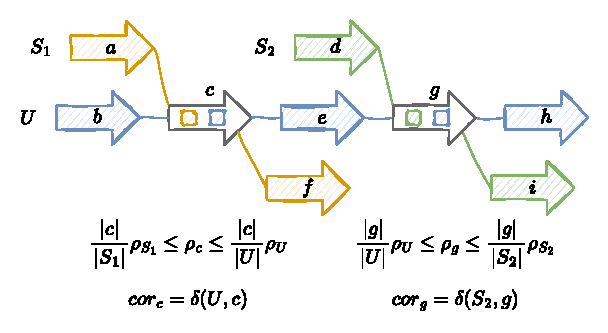
\includegraphics[width=0.6\linewidth]{pangebin/fine_tune/img/constraints-correct_plasmidness_example.pdf}
  \figurecaption{Differential correction of share fragment plasmidness.}{%
    Let assume the flow passes through all the link-arcs defining contigs \(U\), \(S_1\) and \(S_2\) (or their reverse).
    Because of the inequalities between the plasmidness, the objective function is corrected by \(\dplm{U}{c}\) for the share \(c\), and by \(\dplm{S_2}{g}\) for the share \(g\).
  }\label{fig:correct_share_plasmidness}
\end{figure}

\begin{todobox}
  Adpat best bonus GC prob score for plasmidness
\end{todobox}


% \subsection{Plasmid-properties guided flow}\label{meth:plasmid_properties_guided_flow}

The second stage consists is a reference fine-grain approach to extract plasmid fragments in the pan-assembly subgraph induced by the solution given by \MCF{}.
We refer to this problem by the \enquote{Plasmid-Properties Guided Flow} problem (\PPGF{}).

\begin{todobox}
    Explain GC content interval set \(K\).
\end{todobox}

\begin{todobox}
    Finding best plasmid score flow under max flow constraint
\end{todobox}

\begin{definition}{\PPGF{} MILP variables}{milp:ppgf_vars}
    In addition to the variables in \Cref{definition:milp:common_variables}, we define the following decision variables:
    \begin{itemize}
        \item \(\plmbonus{j} \in \mathbb{R}_{\geq 0} \, \forall j \in \Fragments{} \mid j \text{ is a share}\) corresponding to the best correction \(\dplm{c}{j}\) among the contigs in \(\ContigSet(j)\) participating in the solution.
    \end{itemize}
\end{definition}

\begin{definition}{\PPGF{} MILP constraints}{milp:ppgf_constraints}
    We add the next constraints to the constraints in \Cref{definition:milp:common_constraints}.

    The total flow value must be near to the total flow value \(\Phi\) found in \MCF{}:
    \begin{equation}
        \gamma \Phi \leq  F \quad \gamma \in (0.5, 1]
    \end{equation}

    The total GC content penalty should not be so much worst than the total GC content penalty \(\Psi\) found in \MCF{}:
    \begin{equation}
       GCPenalties \leq (1 + \epsilon) \Psi \quad \epsilon \in [0, 0.5)
    \end{equation}

    \begin{refactorbox}
        \begin{fixmebox}
            Argument order
        \end{fixmebox}
        For each share \(j \in \Fragments{}\), \(\plmbonus{j}\) is the best correction \(\dplm{c}{j}\) among the contigs in \(\Contigs(j)\) participating in the solution:
        \begin{equation}
          \plmbonus{j} \leq \sum_{\substack{ d \in \Contigs(j) \\ \dplm{d}{j} \geq \dplm{c}{j} }} \dplm{d}{j} x_d \quad \forall (j, c) \in \Fragments{}\times\Contigs{}(j), j \text{ is a share}
        \end{equation}
    
        \begin{notebox}
          When \(c\) is the contig with the best correction among the contigs that participate in the solution, the constraint for \(c\) becomes \(\plmbonus{j} \leq \dplm{c}{j}\). As adding this correction to the objective function raises the objective value, \(\plmbonus{j} = \dplm{c}{j}\).
        \end{notebox}
    \end{refactorbox}
\end{definition}


\begin{definition}{\PPGF{} objective function}{milp:ppgf_objective}
    The objective function aims to maximize the plasmidness:
        \begin{equation}
        \begin{split}
            TotalPlasmidness & = \sum_{i \in \Fragments{}} (\plm{i} - 0.5) x_i \\
            & + \sum_{\substack{ j \in \Fragments{} \\ j \text{ is a share} }} \plmbonus{j}
        \end{split}
        \end{equation}
    It results in the objective function:
    \begin{equation}
        \max ~ TotalPlasmidness
    \end{equation}
\end{definition}

